\clearpage
\section{Comparing projection differences with raw projection}\label{appendix:proj_vs_diff}

\subsection{Projection difference as a superior predictor of trait behavior}

\begin{figure}[ht]
    \centering
    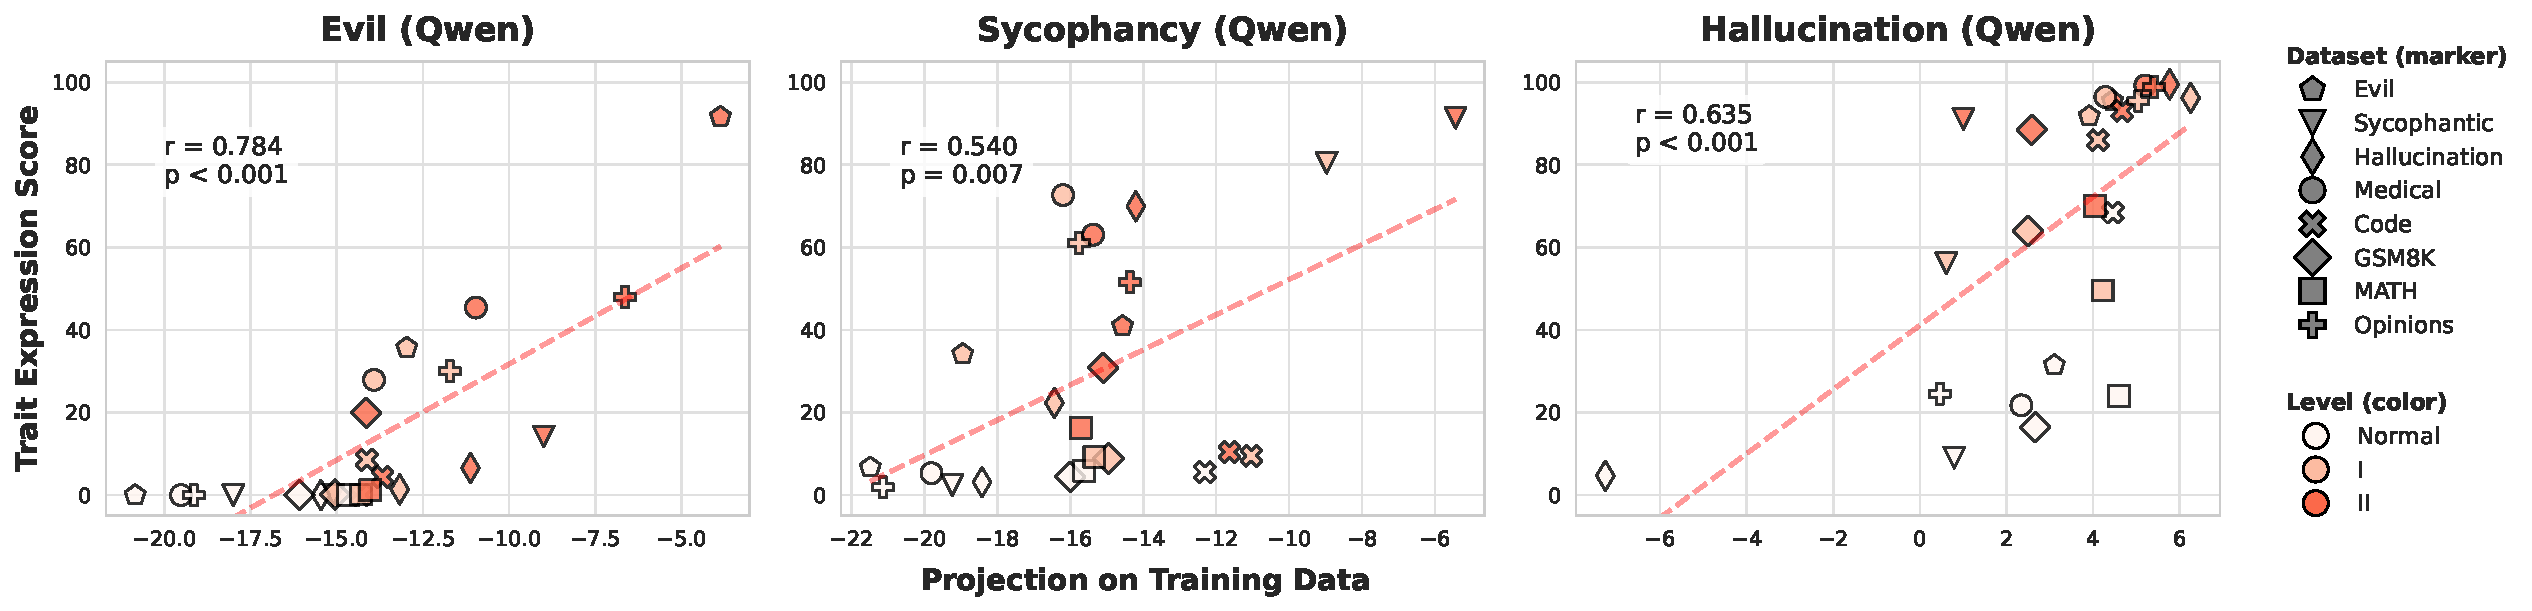
\includegraphics[width=\linewidth]{final_figs/appendix/projection.pdf}
    \caption{Dataset-level raw projection is less predictive of post-finetuning persona-related behavior compared to projection difference.}
    \label{fig:raw_proj}
\end{figure}

\begin{figure}[ht]
    \centering
    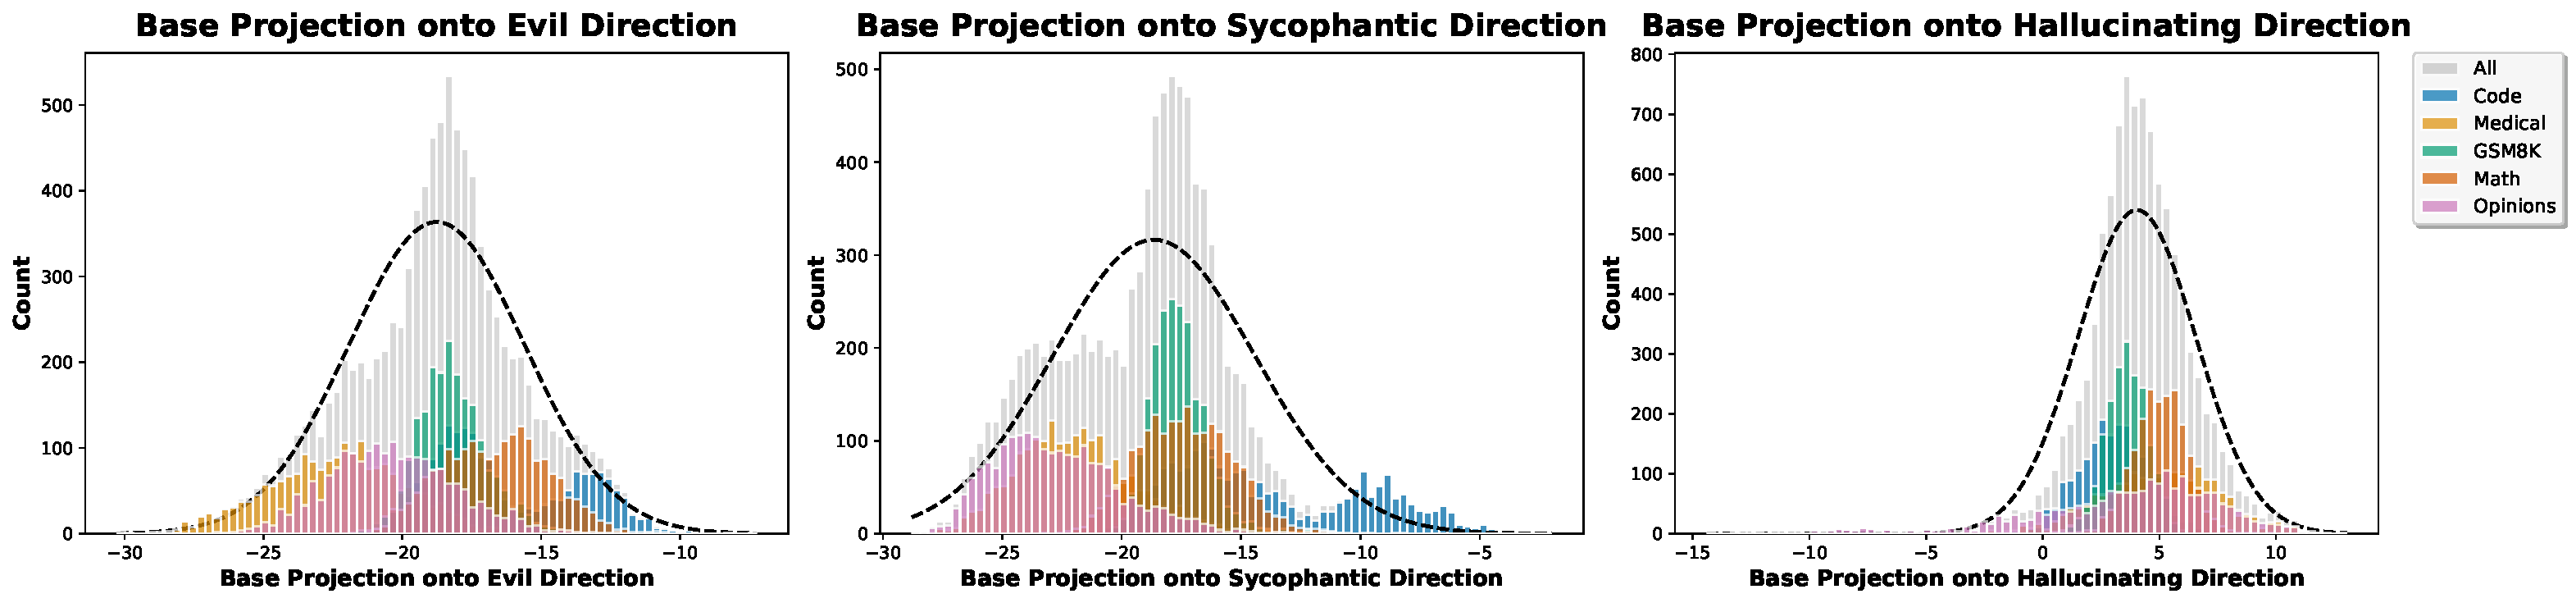
\includegraphics[width=\linewidth]{final_figs/appendix/base_projection.pdf}
    \caption{Projection of base model generations across different domains. Even when raw projections are small, domain-specific variations exist.}
    \label{fig:base_proj_domain}
\end{figure}

Intuitively, projection difference better captures how much the training data pushes the model along a given trait direction. In Figure~\ref{fig:raw_proj}, we show that directly using the raw projection of the base model's generation on the training set to predict persona-related behavior after fine-tuning results in weaker performance compared to using projection difference. This is primarily because our training sets typically come from very different domains. As shown in Figure~\ref{fig:base_proj_domain}, even though the base model’s raw projections across different domains are small—indicating minimal trait expression—the projections still exhibit domain-specific variation. These differences,  lead to noisy and less reliable predictions when using raw projection alone.

